\section{Background} \label{sec:background}

\subsection{Introduction}
Loyalty programs (LPs) have been implemented across the globe to develop brand loyalty by rewarding returning customers. However, current LPs fail to take full advantage of the network effects that can be gained by leveraging blockchain technology. These advantages include increasing customer loyalty, eliminating third party fees through disintermediation, providing data analytics through customer redemption patterns, and leveraging global integration to develop cooperative alliances that span industries and create a more functional LP for both consumers and merchants. 

Koalition is the next generation LP, creating a robust rewards network that integrates existing LPs and adds new opportunities for businesses that previously lacked the resources to deploy their own LP. This network of merchants provides more enticing incentives to customers by allowing them to spend their points when, where and how they want to.  Koalition enables customers to accumulate enough points to redeem for meaningful rewards without the hassle of managing separate accounts for dozens of LPs. For businesses, Koalition makes each rewards point transaction more secure and transparent, while removing trusted third party (TTP) services.

The next sections will first focus on the limitations and problems associated with current rewards programs. Then the utility of blockchain technology will be touched upon before describing how it can be used to disrupt the current loyalty industry. Furthermore, the unique aspects of Koalition?s decentralized attributes, token stability and added benefits will be described in further detail along with a roadmap for future development. 

\subsection{Types of Loyalty Programs}

\subsubsection{Stand-Alone Loyalty Programs}

Customer loyalty is an asset that can be leveraged by both small businesses and big brands. Customers loyal to a particular brand are more likely to spread positive word of mouth, less likely to be swayed by competitors, and are less price sensitive. To better compete in a competitive industry, companies in industries ranging from airlines to supermarkets to local coffee shops create incentives using LPs. These programs offer consumers rewards points proportional to their purchases and allow consumers to accumulate points to redeem different types of rewards. Many companies use LPs to increase customer retention as the cost of acquiring new customers is much greater \cite{VR16}. However, with thousands of programs to choose from, consumers oftentimes are circumscribed by making the most economic travel decisions. According to the $2015$ Colloquy Loyalty Census, the average household belongs to nearly 29 different loyalty programs \cite{CQ15}. This perpetuates frustration because customers either pay high costs for similar services to remain loyal to one LP or they have points scattered among a myriad of LPs that they are unable to redeem for anything worthwhile. The end result is account inactivity and low redemption rates. In fact, the 2016 Bond Loyalty Report which queried 12,000 Americans and 7,000 Canadians about their 280 loyalty programs across various industries, found that only 50\% of them were active members of their respective programs. Of those 50\%, a fifth of them had never redeemed their points. Unredeemed rewards points create accounting liabilities for merchants in the form of unrealized revenues that cannot be absolved until they are redeemed. Furthermore, customer retention rates diminish for LP members who do not redeem their points. These customers are 2.7 times more likely to join a different program altogether \cite{Bond16}. 

Many customers have familiarized themselves with LPs through the travel industry, however, travel companies continue to lose market share to Online Travel Agencies (OTAs). OTAs like Priceline and Expedia act as a one-stop shop for consumers by consolidating the experience of individually booking a flight, hotel, and rental car into one platform. OTAs have their own LPs which give customers more choices (so customers can select the cheapest flight with minimal opportunity costs) and make it increasingly difficult for traditional stand-alone LPs to compete. Airlines, hotels, and rental car companies share up to 20\% of their revenues with OTAs and OTAs are projected to own 41\% of travel industry bookings by 2020 \cite{OTA17}.  Despite this fact, merchants still use OTAs because exiting this channel would result in a significant loss of marketing opportunities.  It is clear that merchants need an alternative loyalty program that provides enough customer flexibility to compete with OTAs, or continue giving up revenue.

\subsubsection{Coalition Loyalty Programs}
While the number of stand-alone LPs have grown, the challenges of these programs to consumers and businesses alike have caused many businesses to search for different LP schemes. Businesses have begun to participate in coalition LPs in an effort to provide customers rewards that can be earned and redeemed faster with greater flexibility across businesses. Most coalition LPs are formed through the agglomeration of existing stand-alone LPs and consist of either pairwise partnerships such as Amex-Uber or centralized partnerships like Starwood Hotels and Resorts (U.S.) and SkyTeam (international alliance). These coalitions help split liability among the participating merchants and partially solve some of the customer frustrations while still attempting to increase customer retention and engagement rates. Furthermore, coalition LPs promote the acquisition of new customers more easily than stand-alone LPs due to inter-company cooperation which favors cross-selling. It costs less to join a coalition LP than to establish a stand-alone program, and empirical evidence shows that businesses in coalition LPs achieve higher marketing performance \cite{VR16}. 

However, coalitions are often times limited in scope. Coalitions typically form among large entities in similar industries (\ie\ the many large hotel, airline, and rental car brands within the travel industry). These coalitions alienate small to medium cap businesses providing complimentary services, and hence fail to leverage the additional network benefits provided by adding these businesses. Furthermore, complex exchange rates and liability transfers between various LPs in a coalition require negotiations that consume unnecessary time and resources. While coalition LPs mark a step forward to fixing the problems that plague stand-alone LPs, these programs have a long way to go to improve customer loyalty and enhance the customer experience.

\subsection{Centralized Databases}
Databases are the primary means by which any digital data and applications are stored. At a high level, these databases consist of a hard drive or series of hard drives whose low level operations (\ie\ where data is stored) is managed by the operating system (Windows, Mac, Linux, etc). A SQL (Structured Query Language) server runs on top of the operating system and is responsible for how the data is accessed, organized, and used. These digital databases are typically centralized and managed by either the business or a TTP. Centralized databases are easy to maintain and simple to implement, but data stored in these databases can be easily manipulated (mutable) by both external and internal actors due to its centralized nature (\ie\ there is a single point of failure). Centralized databases also suffer from increased complexity and maintenance cost as the number of users increase. As users increase, the amount of data stored in the database increases, driving a need for more costly digital space, operational resources, and more IT personnel to manage the database. These problems are significantly magnified for applications that require the interchange and communication of data across different databases. These applications include the formation of consortiums or coalitions in which businesses pool their resources together to achieve a common goal. Generally, centralization introduces a significant amount of friction in these applications because it inhibits modularity (must give control to a central entity, making it difficult to change individual structure), interoperability (different technology, different data structures, etc) and inclusion (difficult, incurs a cost, or slow to add new businesses).

\subsection{The Blockchain}

\subsubsection{Overview}
Blockchain is a novel technology that can address many of the pitfalls of centralized databases. Blockchain can provide an open, distributed database of records acting as a public ledger of all transactions or digital events that have occurred between all participating entities. Essentially, it is a shared database that allows multiple users (who do not trust each other) to transparently and securely modify the database directly to reflect a state change or digital event. This is indeed revolutionary because it enables an ecosystem that distributes the cost and resources to manage and operate a database among all the participants, not just the businesses providing a service. Furthermore, due to the decentralization of the data, a blockchain makes it nearly impossible for external or internal actors to manipulate the data. Indeed, one of the key security features of a blockchain is immutability- once data is stored on the blockchain, it cannot be changed.
%
\begin{framed}
\begin{quote}
\textit{``If TCP/IP is the standard for secure information transfer, then blockchain is the standard for secure value transfer."}
\end{quote}
\end{framed}

Bitcoin \cite{BTC08}, the world's first renowned public blockchain, represents the first use case of blockchain technology by generating value through digital scarcity. In the Bitcoin framework, the exchange of the native cryptocurrency, Bitcoin (BTC), represents a unique transaction. More precisely, consider the following example where John sends 1 BTC to Justin, who subsequently sends 0.5 BTC to Hayden. For simplicity, let us assume that John has 1 BTC in his account, while Justin and Hayden have 0 BTC in theirs. If John sends Justin 1 BTC, John signs a new transaction agreement that deducts 1 BTC from John?s account. This transaction agreement is now worth 1 BTC, and can only be spent by Justin. The transaction agreement between John and Justin (call this $T_1$) is now used to fund this transaction. Justin signs two transaction agreements: one transaction agreement that subtracts 0.5 BTC from $T_1$ and a second transaction agreement (call this $T_2$) with Hayden that is worth 0.5 BTC, which Hayden can spend immediately after the transaction is verified. Thus, in the Bitcoin use case, the blockchain is simply a ledger of unique transactions.

The security foundations of blockchains rely on asymmetric cryptography and distributed consensus \cite{PR17}. Each transaction agreement in the blockchain is protected with a digital signature. John uses his private key to sign the transaction agreement worth 1 BTC with Justin. Justin, using his public key, is then able to independently verify from the digital signature that John authorized the transaction. This prevents a malicious participant from forging a transaction involving John's assets because (s)he must have John?s private key. This transaction (and the transaction between Justin and Hayden) is broadcasted to every participant in the blockchain network in order to be validated and recorded. Transactions are ordered by placing the validated transactions into blocks. These blocks are then linked together to form a chain (hence blockchain) preserving a proper linear, chronological order. For example, the transaction between John and Justin ($T_1$) will always precede the transaction between Justin and Hayden ($T_2$) because any attempts to include $T_2$ in a block where $T_1$ does not precede $T_2$ will be rejected during the validation process (since Justin only has enough BTC to send to Hayden, if John sends it to him first). Note that since every participant is able to manage the blockchain, multiple blocks can be generated by different participants at the same time. In the Proof-of-Work (PoW) scheme, the first participant to solve an extremely difficult cryptographic puzzle will be able to submit their block to the blockchain provided that they prove to everyone in the network that they solved the puzzle. The process of validating the block and the participant's proof that (s)he solved the puzzle forms the consensus portion of the blockchain. Since everyone has the same version of the truth (i.e. same blockchain), it is impossible to change the contents of any block of the chain without getting caught. Furthermore, the difficulty of solving the cryptographic puzzle prevents one person from adding a false block to the chain. Figure \ref{fig:btcfigure} shows a general overview of how blockchains work.
%
\begin{figure}[] % use "t!" to force the float to start the float at top of page
    \centering
        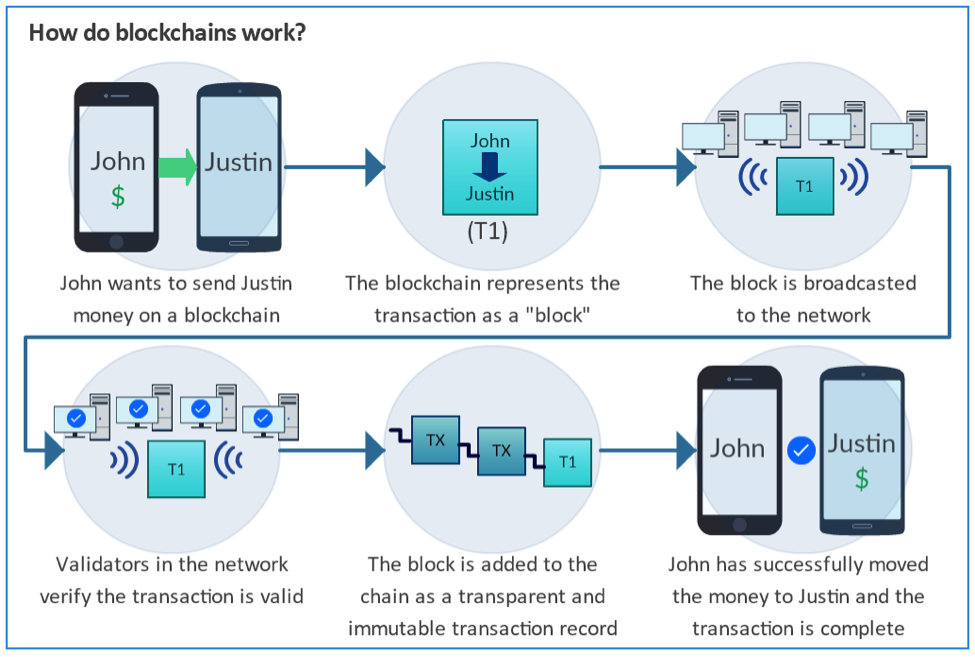
\includegraphics[keepaspectratio, width=0.7\textwidth]{images/blockchains.png}
    \caption{Overview of How Blockchains Work} \label{fig:btcfigure}
\end{figure}

The advent of Bitcoin has helped spawn more advanced blockchain-based platforms. Ethereum \cite{Wood14} is one of these platforms, which allows the implementation of so called smart contracts-- computer programs that control digital assets on the blockchain through a set of arbitrary rules. Smart contracts allow for the complete automation of processes requiring a TTP such as trade agreements, crowdfunding, and redemption of loyalty points. Decentralized applications (Dapps) are client-side applications that allow participants in the blockchain to interact with smart contracts. Dapps and smart contracts enable a dynamic environment for the interaction between participants on the network. Figure \ref{fig:dapps} illustrates the interaction between Dapps and smart contracts.
%
\begin{figure}[h] % use "t!" to force the float to start the float at top of page
    \centering
        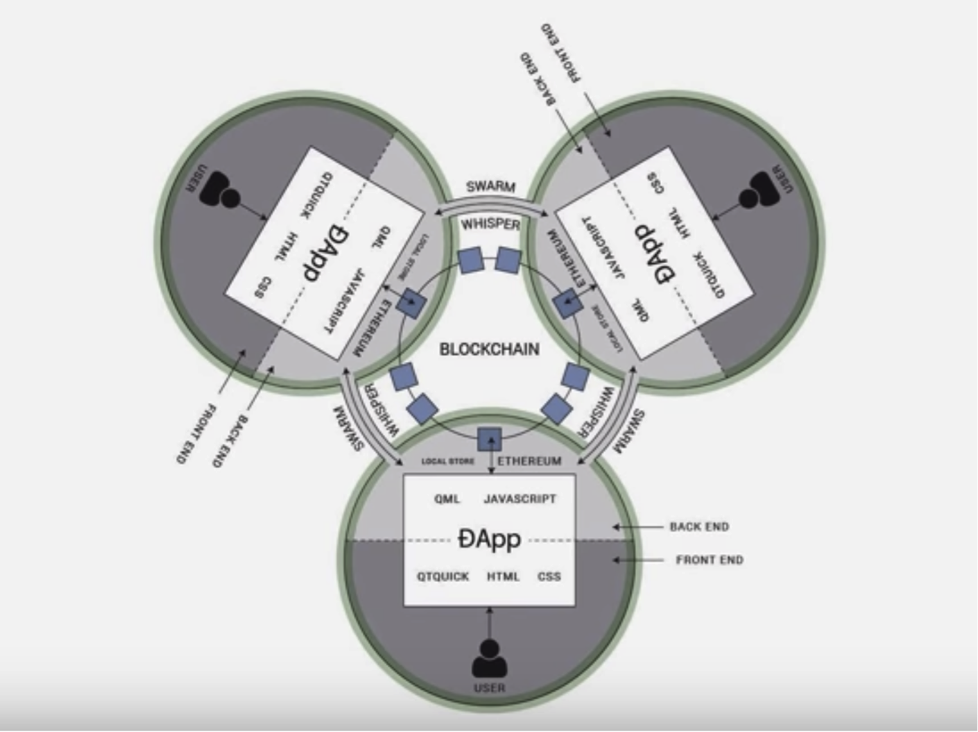
\includegraphics[keepaspectratio, width=0.7\textwidth]{images/dapps.png}
    \caption{Interaction between Dapps and Smart Contracts} \label{fig:dapps}
\end{figure}

Blockchains have seen tremendous growth since the introduction of Bitcoin, and the technology's development has accelerated due to increased adoption by startups and industry alike. For example, the Ethereum project continues to grow as it attempts to solve industry concerns about scaling, customer privacy, and regulation. Alternative blockchain-based platforms such as IBM's Hyperledger Fabric \cite{HL16}, Microsoft's Coco Framework \cite{Coco17}, Multichain \cite{MC16}, and NEM \cite{NEM} address the problem of scaling and customer privacy through permissioned or private blockchains. While these platforms handle a narrower range of use cases, they address some of the major problems raised by industry. Projects, such as Cardano \cite{Cardano}, aim to solve these problems while preserving the complexity of applications that can be run on the blockchain.

\subsubsection{Permissionless vs. Permissioned Blockchains}